\documentclass{article}
\usepackage[utf8]{inputenc}

\title{IF702 - REDES NEURAIS}
\author{Samuel Henrique Vieira Rodrigues}
\date{Novembro 2019}

\usepackage{natbib}
\usepackage{graphicx}

\begin{document}

\maketitle

\section{Introdução}
As redes neurais artificiais foram inspiradas no sistema nervoso central humano, inicialmente o objetivo era que a rede neural fosse capaz de resolver problemas como um cérebro humano. Porém, com o passar do tempo, o foco mudou e as redes neurais passaram a ser utilizadas para resolver problemas específicos. As principais vantagens das redes neurais artificias são: capacidade de aprender, reconhecer padrões e generalizar.

\begin{figure}[h!]
\centering
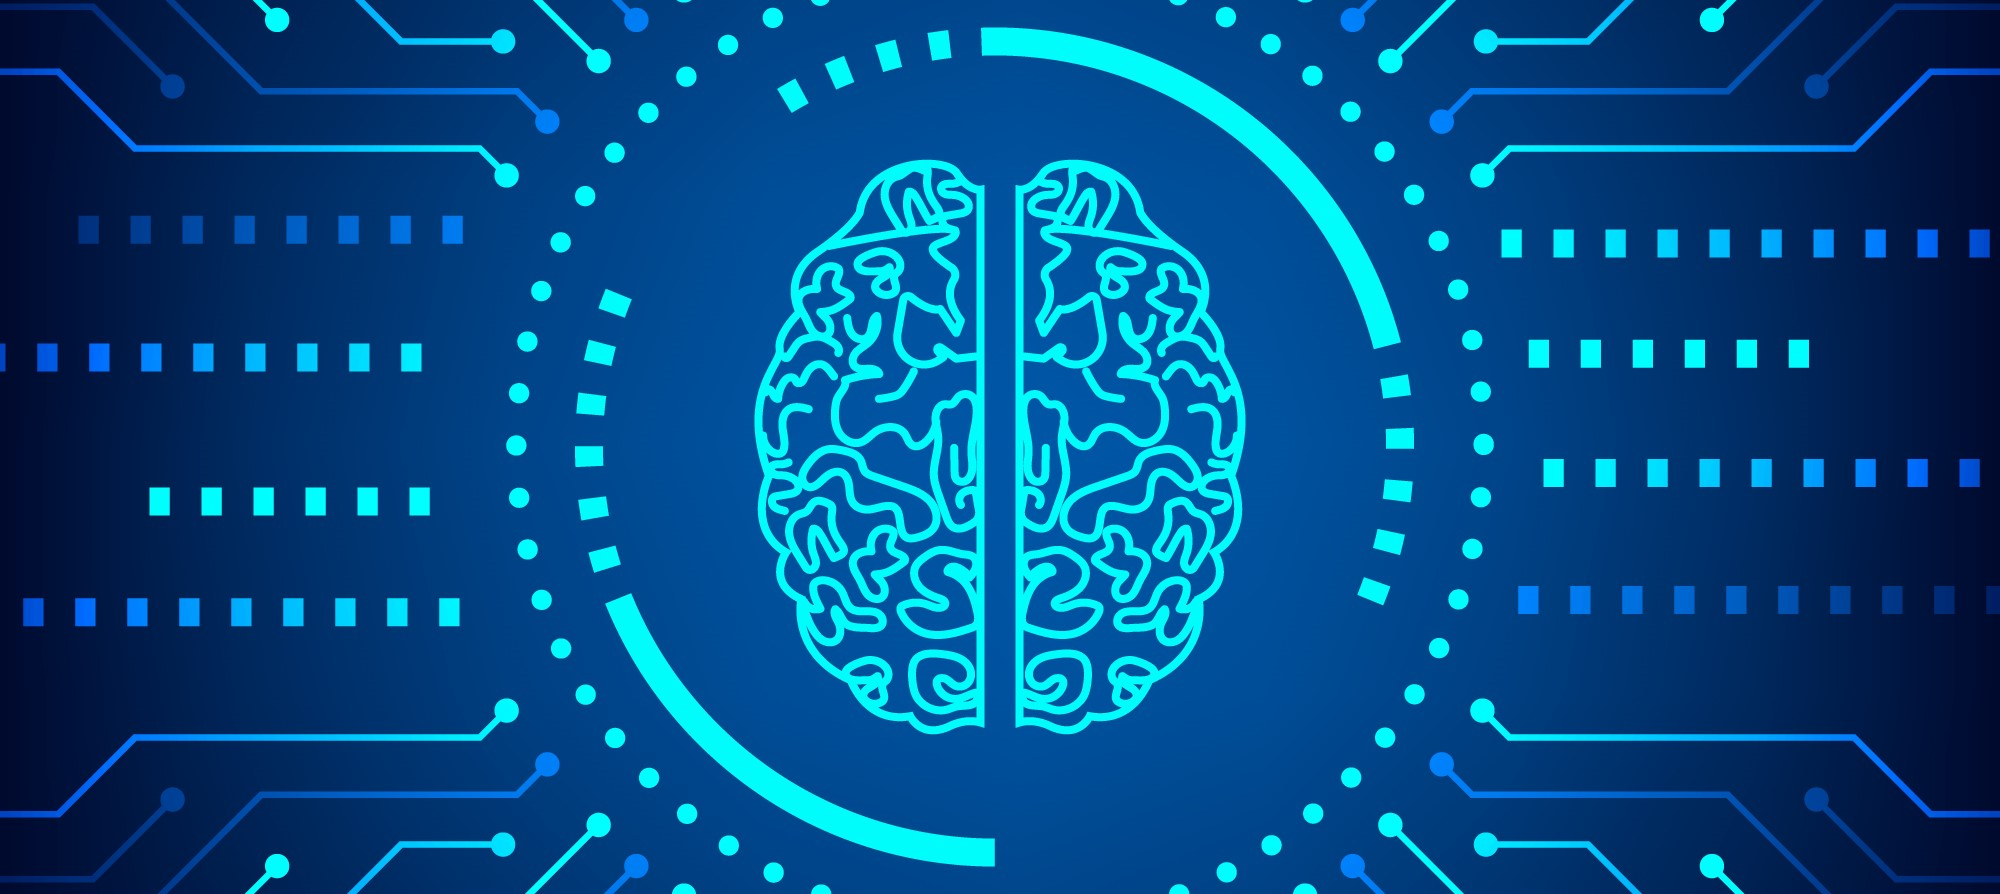
\includegraphics[height=5.2cm]{redes-neurais.jpg}
\caption{Redes Neurais}
\label{fig:redes-neurais}
\end{figure}

\section{Relevância}
As redes neurais artificiais podem agilizar e melhorar processos de decisão em diversas áreas, como:
\begin{itemize}
    \item Reconhecimento de caracteres e de voz (Processamento de Linguagem Natural)
    \item Visão computacional para interpretar fotos e vídeos
    \item Marketing direcionado
    \item Sistemas de controle robóticos
\end{itemize}

\section{Relação com outras disiciplinas}
\begin{itemize}
    \item IF699 - Aprendizagem de Máquina
    \item IF704 - Processamento de Linguagem Natural
    \item IF700 - Percepção Computacional e Reconhecimento de Padrão
    \item IF705 - Automação Inteligente
\end{itemize}

\bibliographystyle{plain}
\bibliography{references}
\end{document}
